\chapter{Crittografia Simmetrica}

\begin{figure}[h]
    \centering
    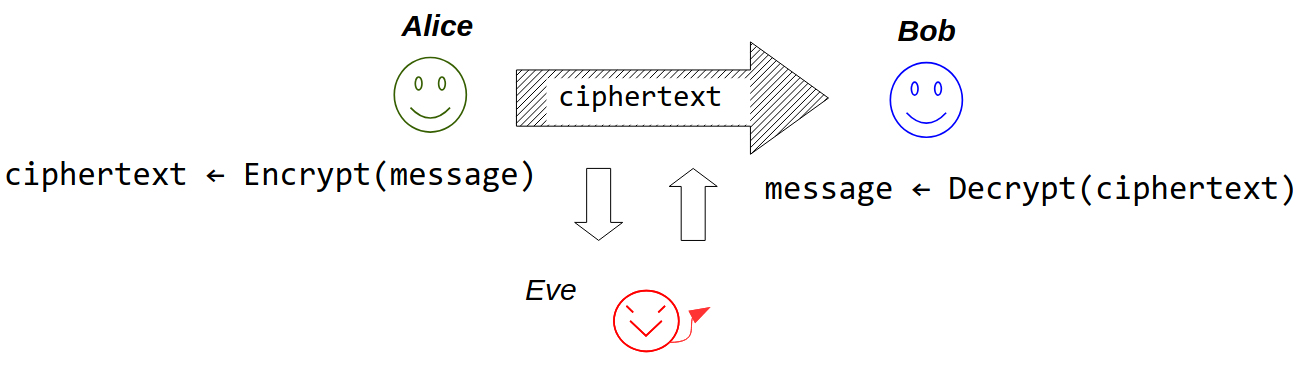
\includegraphics[width=\textwidth]{img/crypto_symm_1.png}
\end{figure}

Le garanzie di sicurezze che si cercano di mantenere sono:
\begin{itemize}[nosep]
    \item \textbf{confidenzialità}: Eve non può accedere a nessuna della informazioni sul messaggio.
    \item \textbf{autenticazione}: Bob può verificare se il messaggio non è stato inviato da Alice, viene anche chiamata \textbf{\textit{data orgin authenticity}} nel contesto della comunicazioni e implica anche la protezione contro modifiche illegittime (\textbf{integrità}).
\end{itemize}

\begin{flushleft}
    La sicurezza non esiste in natura è quindi necessario idearla e modellarla, questa prima parte prende il nome di \textit{Definitional Activity}. È comunque importante ricordare che le \textbf{definizioni} possono essere \textbf{errate} principalmente per errori nella modellazione o nello sviluppo software, ma anche perché non si è stato in grado di modellare quello che era invece richiesto. Un altro errore che si può essere portati a fare è quello di utilizzare in maniera errata certe definizioni ad esempio al di fuori del contesto per cui era stata definita. \newline
    \textbf{\textit{Definitional Activity}}: permette di descrivere che cosa l'avversario può \textbf{fare} e cosa può \textbf{vedere}. Esistono molteplici modi per definire la sicurezza in maniera più formale, uno tra questi è la \textbf{\textit{simulation-based security}} dove viene definita una funzione ideale che soddisfa la definizione di security e poi dimostrare che la funzione costruita si comporti come quella ideale.
\end{flushleft}

\begin{figure}[h]
    \centering
    \begin{large}
        \textbf{\textit{First Adversary Model}} \\
    \end{large}
    Quindi modelliamo e identifichiamo le casistiche e tipologie di un attaccante. \\

    \begin{minipage}[t]{0.50\textwidth}
        \centering
        \begin{boxA}
            \textcolor{red}{\textbf{\textit{Attack Model: Passive Eavesdropper (EAV)}}} \\
            Ha capacità di lettura dei soli \textit{ciphertext} e non è capace di \textbf{scegliere nulla}
        \end{boxA}
    \end{minipage}
    \begin{minipage}[t]{0.45\textwidth}
        \centering
        \begin{boxA}
            \textcolor{red}{\textbf{\textit{Security Goal: Indistinguishably}}} \\
            L'avversario non può distinguere il \textit{ciphertext} da sequenza di caratteri random.
        \end{boxA}
    \end{minipage}
\end{figure}

\begin{flushleft}
    Modellando in questo modo il nostro avversario è possibile osservare che non viene descritto nulla sul nascondere la lunghezza del \textit{plaintext}, infatti per questa prima modellazione l'avversario può vedere la lunghezza del \textit{plaintext}. \\
    \textbf{Nota}: la crittografia non ha come obiettivo quello di nascondere la lunghezza del testo in chiaro, nel caso in cui questa informazione fosse confidenziale, è necessario proteggerla a livello applicativo.
\end{flushleft}

\begin{flushleft}
    Le capacità di un avversario vengono espresse e descritte tramite degli algoritmi chiamati \textbf{esperimenti}, che vengono eseguiti da un'entità chiamata \textbf{\textit{challenger}} (che per semplicità andiamo ad identificare nell'attore onesto). \\
    Come prima andiamo ad analizzare \textbf{\textit{IND-EAV}}, il \textit{challenger} va a scegliere un messaggio \textbf{m} che viene scelto con la stessa probabilità tra:
    \begin{itemize}[nosep]
        \item dati random: $m \leftarrow \{0, 1\}^n$
        \item un messaggio generato attraverso la cifrazione $m = \text{Encryption}(p)$, dove \textbf{p} può essere scelto nello stesso modo di prima $p \leftarrow \{0, 1\}^n$
    \end{itemize}
    All'avversario viene fornito \textbf{m} e deve scegliere se è un messaggio randomico o se è l'output dell'\textit{encryption}, l'avversario vince l'esperimento se la sua decisione è corretta.
\end{flushleft}

\begin{flushleft}
    \textcolor{red}{\textbf{\textit{IND-EAV: Perfect \& Computational Indistinguishably}}} \\
    Andremo a discutere due tipologie di sicurezza:
    \begin{enumerate}[nosep]
        \item \textbf{\textit{perfect}}: la probabilità dell'avversario di vincere l'esperimento è del \textbf{50\%}, viene anche chiamata \textbf{\textit{Unconditional Security}} o \textbf{\textit{Informatition Theoretic Security}}.
        \item \textbf{\textit{computational}}: la probabilità dell'avversario di vincere l'esperimento è \textbf{50\%} più una \textbf{quantità trascurabile}.
    \end{enumerate}
    Qualunque tipologia di schema \textbf{praticabile} garantisce \textbf{sicurezza computazionale}, e se capace di essere sicuro contro un'\textbf{esperimento IND-EAV} viene detto \textbf{\textit{IND-EAV secure}}.
\end{flushleft}

\section{Sicurezza Incondizionata \& One-Time Pad}
\textcolor{red}{\textbf{XOR}}: gli schemi di crittografia moderni sono progettati per \textbf{dati binari}. L'operazione base per la crittografia simmetrica è lo \textbf{XOR}.

\begin{center}
    \begin{minipage}[c]{0.3\textwidth}
        \centering
        $c = m \oplus k$
    \end{minipage}
    \begin{minipage}[c]{0.3\textwidth}
        \centering
        \begin{tabular}{|c|c|c|}
            \hline
            \textbf{m} & \textbf{k} & \textbf{c} \\ \hline
            0 & 0 & 0 \\ \hline
            0 & 1 & 1 \\ \hline
            1 & 0 & 1 \\ \hline
            1 & 1 & 0 \\ \hline
        \end{tabular}
    \end{minipage}
    \begin{minipage}[c]{0.3\textwidth}
        \centering
        \textbf{Nota}: lo \textbf{XOR} può essere anche modellato come la somma bit per bit modulo 2: $c_i = (m_i \oplus k_i) \; \text{mod} \; 2$
    \end{minipage}
\end{center}

\begin{flushleft}
    Lo XOR viene scelto perché dato un certo \textbf{m}, se \textbf{k} viene scelta in maniera randomica la probabilità di \textbf{c} di essere \textbf{0} o \textbf{1} è \textbf{p = 0.5}. \\
    In questo modo sapere \textbf{c} non da informazioni su \textbf{m} e quindi \textbf{c} è indistinguibile da una successioni di bit random: $\{0, 1\}^n$
\end{flushleft}

\begin{flushleft}
    \textcolor{red}{\textbf{\textit{One-Time Pad - Vernam's Cipher}}}: è un algoritmo di crittografia che esegue un XOR bit a bit tra il testo in chiaro e la chiave, le due lunghezze devono essere uguali e la chiave devere essere random. $c_i = m_i \oplus k_i \; \forall i \in \{0, ..., n\}$ dove $n$ è la lunghezza del testo in chiaro. \\
    Per la decifrazione bisogna utilizzare la stessa chiave: $m = c \oplus k = (m \oplus k) \oplus k = m \oplus (k \oplus k) = m$. \\
    Anche se \textbf{OTP} è \textbf{incondizionatamente sicuro} non è praticabile realmente in quanto la generazione della chiave per testo arbitrario è computazionalmente onerosa ed è un algoritmo completamente \textbf{malleabile}. Gli schemi di crittografia oggi usati sono \textbf{computazionalmente sicuri}.
\end{flushleft}

\begin{flushleft}
    \textcolor{red}{\textbf{Nota sulla randomicità in crittografia}}: la randomicità in crittografia è differente da quella ``statistica'', ovvero una \textbf{distribuzione uniforme di 0 e 1} (che è necessaria ma non sufficiente), ma deve essere \textbf{\textit{unpredictable}}, in modo tale che anche osservando una sequenza, più o meno lunga di bit, non sia possibile predirre il bit successivo.
\end{flushleft}

\section{Sicurezza Computazionale: Security Level e Key Sizes}
Gli schemi crittografici moderni hanno come parte dei requisiti i \textbf{\textit{Kerckhoffs principle}} e necessitano uno \textbf{spazio delle chiavi largo} abbastanza per prevenire attacchi di ricerca esaustiva. Inoltre lo schema deve essere progettato in modo che si possa prevenire crittanalisi sul crittogramma, quindi nessuna informazione deve essere ottenuta dal crittogramma indipendentemente dal tipo di dato e deve essere sicura contro l'esperimento IND-EAV. 

Le condizioni necessarie avere degli schemi computazionalmente sicuri sono:
\begin{itemize}[nosep]
    \item gli schemi utilizzati devono essere computazionalmente sicuri.
    \item definiamo $F_k$ come una \textbf{PRF - \textit{Pseudo-Random Function}} con una chiave fissa \textbf{k} scelta randomicamente.
    \begin{itemize}[nosep]
        \item la \textbf{chiave} deve essere ``\textbf{corta}'' (ma lunga abbastanza per resistere ad attacchi a forza bruta).
        \item deve essere capace di cifrare grandi moli di dati.
        \item data la \textbf{chiave} le funzioni di \textbf{\textit{encryption}} e \textbf{\textit{decryption}} devono essere \textbf{efficenti}.
        \item senza la \textbf{chiave} la probabilità di rompere lo schema crittografico deve essere \textbf{trascurabile}.
    \end{itemize}
\end{itemize}

\begin{flushleft}
    È necessario tradurre in termini algoritmici \textbf{efficenti} e \textbf{trascurabile}. Alice e Bob che usano la funzione di \textit{encryption} e \textit{decryption} con la chiave devono essere capaci di eseguire gli algoritmi con costo \textit{efficient}, quindi il \textbf{costo computazionale} e \textbf{di memorizzazione} sono \textbf{polinomiali} sui parametri di sicurezza. Eve, che non conosce la chiave deve operare in maniera attraverso algoritmi \textbf{inefficienti}. \\
    $\rightarrow$ se il costo dell'attacco diverge da quello degli attori legittimi, è possibile scegliere i parametri di sicurezza appropriati in modo tale che la probabilità di completare correttamente l'algoritmo si molto piccola: \textbf{trascurabile}. 
\end{flushleft}

\begin{flushleft}
    Se fissiamo come probabilità di successo per definire un attacco a \textit{brute force} \textbf{inefficiente} $10^{-6}$, identifichiamo il valore di \textbf{N} per funzioni che hanno costo computazionale diverso, per quali valori di \textbf{n > N} le probabilità di sucesso sono inferiori?

    \begin{center}
        \begin{tabular}{lllll}
            \textbf{Costo di Esecuzione} && \textbf{Probabilità di Successo} && \textbf{\textit{Threshold}, b = 2} \\
            $\mathbf{O}(b^n)$ & $\rightarrow$ & $\mathbf{O}(b^{-n})$ & $\rightarrow$ & \textbf{N = 20} \\
            $\mathbf{O}(b^{\sqrt{n}})$ & $\rightarrow$ & $\mathbf{O}(b^{- \sqrt{n}})$ & $\rightarrow$ & \textbf{N = 400} \\
            $\mathbf{O}(b^{\log n})$ & $\rightarrow$ & $\mathbf{O}(b^{- \log n})$ & $\rightarrow$ & \textbf{N = 32}
        \end{tabular}
    \end{center}
    La conoscenza del costo dell'attacco più noto determina il valore del parametro di sicurezza, tra gli altri, la \textbf{dimensione della chiave}, identificato dal valore \textbf{N}.

    {\centering
        $\exists N \; | \; f(n) < \frac{1}{p(n)}, \; \forall n < N$
    \par}
\end{flushleft}

\begin{boxA}
    \textcolor{orange}{\textbf{Esempio}} \\
    Definiamo il costo di cifrazione $c_{enc}(n) = n$ mentre il costo dell'attacco $c_{attack} = n^2$ dove $n$ è la lunghezza della chiave. \\
    Negli anni 2000 l'\textit{encryption} utilizzava una chiave a 64bit e impiegava 1ms, mentre l'attacco a forza bruta, impiegava 2 anni. Dopo 10 anni, nel 2010, con la stessa chiave la cifrazione impiegava 0.1ms e il suo brute force 2 mesi. \\ \newline
    Aumentando la lunghezza della chiave, raddoppiandola, la fase di cifrazione impiegava 0.2ms, mentre quella di \textit{brute force} passava da $2^{64}$ a $2^{128} \simeq 10^{20}$ mesi.
\end{boxA}

\begin{flushleft}
    Grazie a nuove scoperte vengono trovati algoritmi che \textbf{indeboliscono} o \textbf{compromettono} il cifrario. Ad esempio alcuni schemi vengono pubblicamente violati pochi anni dopo la loro scoperta come gli schemi crittografici della famiglia \textit{rc} o \textit{sha1}. È anche possibile che schemi standard vengano indeboliti attraverso \textit{backdoor}, parametri deboli o ``particolari'' e implementazioni deboli.
\end{flushleft}

\begin{flushleft}
    \textcolor{red}{\textbf{\textit{Efficient function}}} $\rightarrow$ \textbf{\textit{polynomial}} \\
    Il costo (computazionale e memorizzativo) sono polinomiali rispetto ad un certo parametro di sicurezza $n$, algoritmi di \textit{encryption} costano al massimo: 
    
    {\centering
        $p(n) := a \cdot n^x$
    \par}

    \textcolor{red}{\textbf{\textit{Negligible function}}} $\rightarrow$ \textbf{\textit{smaller that any inverse polynomial}} \\
    Esiste un valore di \textbf{N} tale che la funzione sia minore di qualsialsi funzione polinomiale:

    {\centering
        $\exists N \; \text{t.c.} \; f(n) < \frac{1}{p(n)}, \; \forall \; n < N$
    \par}
\end{flushleft}

\begin{flushleft}
    \textcolor{red}{\textbf{\textit{PseudoRandom functions}}} \\
    Definiamo una \textbf{funzione ideale} che soddisfa computazionalmente l'esperimento di sicurezza IND-EAV, nel caso di crittografia a chiave privata, questo tipo di funzione si chiama \textbf{\textit{(keyed) family of PseudoRandom Function (PRF)}}.

    {\centering
        $\mathbf{F} \; : \; \mathbf{K} \times \mathbf{P} \mapsto \mathbf{C}$
    \par}

    Dove:
    \begin{itemize}[nosep]
        \item \textbf{K} è uniformemente scelto da $\{0, 1\}^{Lk(n)}$
        \item \textbf{P} è il \textit{plaintext} scelto arbitrariamente da $\{0,1\}^{Lp(n)}$
        \item \textbf{C} soddisfa computazionalmente \textbf{IND-EAV}, dove la ``quantità trascurabile'' è espressa dalla funzione \textbf{negl(n)} 
    \end{itemize}

    Uno schema di crittografia deve essere \textbf{funzionale}. Definiamo \textbf{F} come la \textbf{PRF} allora \textbf{F} si definirà computazionalmente sicura se:
    \begin{itemize}[nosep]
        \item lo spazio della chiavi è ``\textbf{piccolo}'', ma grande a sufficienza per resistere ad attacchi basati su ricerca esaustiva. Quindi $Lk(n)$ \textbf{deve} essere una funzione efficiente.
        \item ha la capacità di generare in output grande quantità di dati \textbf{\textit{pseudorandom}} (è sicuro per IND-EAV).
        \item il costo di computazione di \textbf{F} è \textbf{efficiente}.
        \item senza la chiave, la probabilità di rompere lo schema crittografico è \textbf{trascurabile}, il costo di calcolare $\mathbf{F}^{-1}$ è \textbf{inefficiente}.
    \end{itemize}
\end{flushleft}

\begin{flushleft}
    \textcolor{red}{\textbf{\textit{Concrete parameters for acceptable security guarantees}}} \\
    Gli schemi di crittografia (simmetrica) moderni vengono considerati computazionalmente sicuri, tali schema possono essere violati se si dispone di abbastanza tempo e abbastanza risorse. \\
    Il \textbf{\textit{Security Level}} dello schema è la media del numero di operazioni necessarie per rompere lo schema: gli standard stabiliscono dei valori tali che la quantità di tempo e risorse necessaria per calcolare tale quantità di operazioni è \textit{unfeasible}.
    \begin{itemize}[nosep]
        \item 80-bit di sicurezza $\rightarrow \; 2^{80}$ operazioni in media per rompere lo schema (insicuro dal 2010).
        \item 112-bit di sicurezza $\rightarrow \; 2^{112}$ operazioni in media per rompere lo schema (insicuro dal 2030).
        \item 128-bit di sicurezza $\rightarrow \; 2^{128}$ operazioni in media per rompere lo schema (stimata la sicurezza per ogni scenario successivo).
    \end{itemize}

    Nei moderni \textbf{schemi di crittografia simmetrica}, la \textbf{lunghezza della chiave} definisce il \textbf{livello di sicurezza}, in quanto l'attacco \textit{best-known} è basato sull'indovinare il segreto. A differenza, negli \textbf{schemi di crittografia asimmetrica} dove invece è presente solo una correlazione, in quanto dipende dagli attacchi noti alla matematica sottostante. \\

    Software e librerie \textbf{dovrebbero} implementare configurazioni \textbf{sicure} di \textbf{default} e aggiornate se necessarie
\end{flushleft}

\begin{flushleft}
    \textcolor{red}{\textbf{\textit{Asymmetric Cryptography \& Quantum Computers (PQC)}}} \\
    Si stima che gli attuali standard di crittografia asimmetrica saranno efficacemente violati dai computer quantistici nei prossimi decenni. Nell'ultimo decennio, sono stati ipotizzati e analizzati a fondo nuovi problemi cosiddetti ``\textbf{\textit{post-quantum hard problems}}'', ovvero che non possono essere risolti in modo efficiente nemmeno con un computer quantistico.
\end{flushleft}

\section{Stream Cipher}
Il primo approccio per implementare una funzione ``reale'' che approssimi la funzione ideale PRF. Gli \textit{stream cipher} sono \textbf{\textit{Deterministic Pseudorandom Bitstring Generators (DPBG)}}. Gli schemi a flusso sono funzioni \textbf{deterministiche} che prendono in input \textbf{\textit{small random input}} e generano come output dati che non possono essere distinti (\textbf{\textit{indistinguishably}}) da dati random e non su cui non si può fare una previsione (\textbf{\textit{unpredictable}}), il dato \textbf{pseudo-random} viene chiamato \textbf{\textit{keystream}}, la funzione di cifrazione richiede xor\textit{are} il \textit{keystream} con il messaggio, infatti gli \textit{stream cipher} cercano di approssimare il \textbf{OTP}

\begin{figure}[h]
    \centering
    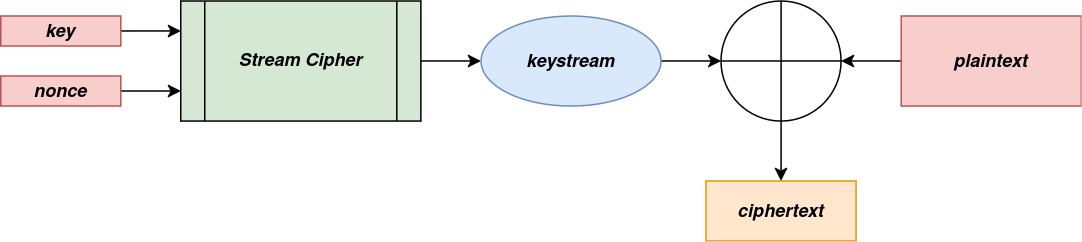
\includegraphics[width=\textwidth]{img/stream_cipher}
    \label{fig:stream_cipher}
\end{figure}

\begin{flushleft}
    Il \textbf{\textit{nonce}} è un valore non confidenziale che \textbf{deve} essere \textbf{univoco} per ogni operazioni di \textit{encryption}. \\
    Uno dei più popolari cifrari a flusso è \textbf{\textit{ChaCha20}}, utilizzo:
    \begin{lstlisting}[language=bash]
    $ echo Hello! | openssl chacha20 -pbkdf2 -k pippo -a -e | \
        openssl chacha20 -pbkdf2 -k pippo -a -d
    \end{lstlisting}

    Questa tipologia di schema è \textbf{malleabile} ed è vulnerabile a \textbf{riutilizzo della chiave}, sia in caso di messaggi diversi che nel caso di due stati diversi di un certo file (dipende dal contesto)

    {\centering
        $c_1 = m_1 \oplus \text{DPGB}(k) \qquad c_2 = m_2 \oplus \text{DPGB}(k)$ \\
        $c_1 \oplus c_2 = (m_1 \oplus \text{DPGB}(k)) \oplus (m_2 \oplus \text{DPGB}(k)) = (m_1 \oplus m_2) \oplus (\text{DPGB}(k) \oplus \text{DPGB}(k)) = m_1 \oplus m_2$
    \par}

    In questo modo la \textit{keystream} viene generata in modo che dipenda unicamente dalla chiave, se noi andiamo a ad utilizzare un altro valore (\textbf{\textit{nonce}}) è possibile rimuovere la vulnerabilità di riutilizzo della chiave. Definendo $k_i$ la \textit{keystream} nell'istante $i$-esimo avremo:

    {\centering
        $k_i = \text{DPBG}(k, n)$
    \par}
    Dove:
    \begin{itemize}[nosep]
        \item \textbf{k} è la chiave privata della comunicazione.
        \item \textbf{n} è il \textbf{nonce}, il problema permane se nessuno dei due viene aggiornato.
    \end{itemize}
\end{flushleft}

\begin{flushleft}
    \textcolor{red}{\textbf{\textit{Trasparent Data Encryption (TDE)}}} \\
    Nel caso in cui si voglia cifrare un disco, si vuole non inficiare lo spazio totale che si ha, quindi per evitare che il nonce venga salvato per ogni porzione scritta su disco normalmente si tende ad utilizzare informazioni che esistono già. \\
    Il contesto non può essere utilizzato in quanto nel tempo non cambia mai quindi si è comunque affetti da \textit{key reuse}.
\end{flushleft}

\section{Block Cipher \& Modes of Operation}
Un \textbf{cifrario a blocchi} è una famiglia di permutazioni pseudo-causali con chiave [\textbf{\textit{keyed family of pseudorandom permutation (PRP)}}].

{\centering
    $\mathbf{F} \; : \; \{0, 1\}^{Lk} \times \{0, 1\}^{Lb} \mapsto \{0,1\}^{Lb}$
\par}

\begin{flushleft}
Dove \textbf{Lb} è la lunghezza del blocco da cifrare, mentre \textbf{Lk} è la lunghezza della chiave. Nei \textit{block cipher} sia la funzione $F$ che $F^{-1}$ sono \textbf{efficenti}.
\end{flushleft}

\begin{boxA}
    \textcolor{orange}{\textbf{Esempio}}: consideriamo un \textit{block cipher} ideale che utilizza una permutazione dell'alfabeto, per mappare ogni carattere, che è noto in crittografia classica come \textbf{\textit{substitution cipher}}.
    \begin{center}
        \begin{tabular}{p{0.2cm}p{0.2cm}p{0.2cm}p{0.2cm}p{0.2cm}p{0.2cm}p{0.2cm}p{0.2cm}p{0.2cm}p{0.2cm}p{0.2cm}p{0.2cm}p{0.2cm}p{0.2cm}p{0.2cm}p{0.2cm}p{0.2cm}p{0.2cm}p{0.2cm}p{0.2cm}p{0.2cm}p{0.2cm}p{0.2cm}p{0.2cm}p{0.2cm}p{0.2cm}}
            \textbf{A} & \textbf{B} & \textbf{C} & \textbf{D} & \textbf{E} & \textbf{F} & \textbf{G} & \textbf{H} & \textbf{I} & \textbf{J} & \textbf{K} & \textbf{L} & \textbf{M} & \textbf{N} & \textbf{O} & \textbf{P} & \textbf{Q} & \textbf{R} & \textbf{S} & \textbf{T} & \textbf{U} & \textbf{V} & \textbf{W} & \textbf{X} & \textbf{Y} & \textbf{Z} \\
            H & L & S & T & G & R & I & J & V & F & U & K & D & M & Z & B & P & A & E & W & N & Y & Y & X & Q & C \\
        \end{tabular}
    \end{center}
    La mappatura delle lettere è la chiave del nostro cifrario e la lunghezza della chiave è pari a:

    {\centering
        $26 \cdot \log_2 26 \simeq 112 \; \text{bits}$
    \par}
\end{boxA}

\begin{boxA}
    \textcolor{orange}{\textbf{Esempio: \textit{Ideal Block Cipher} con \textit{block size} 2}} \\
    In questo caso andiamo a mappare ogni possibile valore di due bit $2^2 = 4$ con ogni possibile permutazione dei suoi valori $4! = 24$ e utilizziamo l'\textbf{indice} come chiave che va a selezionarci la permutazione associata.
    \begin{center}
        \renewcommand{\arraystretch}{0.7}
        \begin{tabular}{c|cccc}
            \textbf{Indice} & \textbf{00} & \textbf{01} & \textbf{10} & \textbf{11} \\ \hline
            \textbf{0}  & 00 & 01 & 10 & 11 \\
            \textbf{1}  & 00 & 01 & 11 & 10 \\
            \textbf{2}  & 00 & 10 & 01 & 11 \\
            \textbf{3}  & 00 & 10 & 11 & 01 \\
            \textbf{4}  & 00 & 11 & 01 & 10 \\
            \textbf{5}  & 00 & 11 & 10 & 01 \\
            \textbf{6}  & 01 & 00 & 10 & 11 \\
            \textbf{7}  & 01 & 00 & 11 & 10 \\
            \textbf{8}  & 01 & 10 & 00 & 11 \\
            \textbf{9}  & 01 & 10 & 11 & 00 \\
            \textbf{10} & 01 & 11 & 00 & 10 \\
            \textbf{11} & 01 & 11 & 10 & 00 \\
            \textbf{12} & 10 & 00 & 01 & 11 \\
            \textbf{13} & 10 & 00 & 11 & 01 \\
            \textbf{14} & 10 & 01 & 00 & 11 \\
            \textbf{15} & 10 & 01 & 11 & 00 \\
            \textbf{16} & 10 & 11 & 00 & 01 \\
            \textbf{17} & 10 & 11 & 01 & 00 \\
            \textbf{18} & 11 & 00 & 01 & 10 \\
            \textbf{19} & 11 & 00 & 10 & 01 \\
            \textbf{20} & 11 & 01 & 00 & 10 \\
            \textbf{21} & 11 & 01 & 10 & 00 \\
            \textbf{22} & 11 & 10 & 00 & 01 \\
            \textbf{23} & 11 & 10 & 01 & 00 \\
        \end{tabular}
    \end{center}
    Una tabella è un \textbf{\textit{block cipher} ideale}, quindi se volessimo generalizzare nel caso di una tabella a $n$ bit, quanti bit servirebbero per memorizzarla:
    \begin{itemize}[nosep]
        \item trasferendo unicamente la permutazione unica del blocco a $n$ bit avremo bisogno di $n \cdot 2^n$ bit, il che è un costo esponenziale.
        \item trasferendo l'intera tabella, avremo bisogno di $n \cdot 2^n \cdot 2^n !$ bit il che la renderebbe impraticabile da gestire.
    \end{itemize}
\end{boxA}

\begin{flushleft}
    \textcolor{red}{\textbf{\textit{Encryption schemes} basati su \textit{Block cipher}}} \\
    I \textit{block cipher} sono \textbf{primitive} crittografiche che possono essere utilizzate per costruire degli \textbf{schemi di crittografia simmetrica} (\textit{block cipher $\neq$ encryption scheme}). \\
    I \textit{block cipher} possono essere utilizzati direttamente con \textit{encryption scheme} solo \textbf{in certi casi particolari} (\textbf{KEM}), negli altri casi per costruire uno schema crittografico è necessario un ulteriore algoritmo chiamato \textbf{\textit{operations modes}} (\textit{encryption mode}).
    \begin{itemize}[nosep]
        \item \textbf{AES}: è un \textit{block cipher} che ha una \textbf{\textit{block size}} di 128bits e una \textbf{\textit{key size}} che può variare a 128bits, 192bits, 256bits.
        \item \textbf{AES-128}: una particolare implementazione di \textbf{AES} con la \textit{key size} a 128bits.
        \item \textbf{AES-128-CBC}: è un \textbf{\textit{encryption scheme}} che si basa su un \textit{block cipher} \textbf{AES-128} usato in combinazione con l'\textit{operations mode} \textbf{CBC}.
    \end{itemize}

    \textcolor{red}{\textbf{\textit{Real Block Ciphers}}}: distribuire un algoritmo invece che una tabella è molto più ``facile''. Possibili \textit{block cipher}:

    \begin{center}
        \begin{tabular}{|c|c|c|c|c|} \hline
            \textbf{\textit{block cipher}} & \textbf{\textit{block size}} & \textbf{\textit{key size}} & \textbf{supporto hardware} & \textbf{deprecato} \\ \hline
            DES & 64 bits & 56 bits & si & si \\ \hline
            AES & 128 bits & 128, 192, 256 bits & si & no \\ \hline
            3DES & 64 bits & 56 bits x 3 & si & ni \\ \hline
        \end{tabular}
    \end{center}
    \textbf{AES-NI} mette a disposizione nuove instruzioni hardware per la crittografia tramite \textbf{AES} è diffuso per tutte le CPU x86. \textbf{ARMv8 Cryptography Extensions} che invece non è disponibile su CPU ARM vecchie o di ``fascia bassa''. \\

    \bigskip
    
    Un \textbf{\textit{block cipher}} deve essere progettato basandosi su due proprietà:
    \begin{enumerate}[nosep]
        \item \textbf{Diffusione}: ogni bit del testo in chiaro influsci su ogni bit del crittogramma (durante la modifica).
        \item \textbf{Confusione}: i pattern all'interno del testo in chiaro non influenzano i pattern del testo cifrato.
    \end{enumerate}

    \textbf{Nota}: i \textbf{\textit{block ciphers}} possono lavorare come \textbf{primitive} all'interno di altri blocchi di crittografia, ad esempio \textbf{ChaCha20} e \textbf{SHA2} utilizzano al loro interno dei \textit{block cipher}.
\end{flushleft}

\begin{flushleft}
    \textcolor{red}{\textbf{\textit{Block cipher Operation Modes}}} \\
    Abbiamo detto che \textit{block cipher} sono primitive non schemi di crittografia, infatti sono utilizzabili unicamente su dati che hanno come lunghezza massima la \textit{block size}. Un \textit{block cipher} è \textbf{deterministico}, il che lo rende vulnerabile a \textbf{\textit{frequency attack}}, è però possibile creare uno \textit{symmetric encryption scheme} utilizzando un \textbf{\textit{modes of operations}}. È Possibile suddividerli in famiglie in base al loro comportamento:
    \begin{itemize}[nosep]
        \item costruire un \textbf{\textit{stream cipher}} da un \textit{block cipher}.
        \item cifrare blocco per blocco per ridurlla la \textbf{malleabilità}.
        \item combinare la \textbf{riservatezza} con altre operazioni crittografiche, ad esempio garantire \textbf{integrità}: \textbf{\textit{authenticated encryption}}.
    \end{itemize}
\end{flushleft}

\begin{flushleft}
    \textcolor{red}{\textbf{\textit{Mode of Operation - Electronic CodeBook (ECB)}}}

    {\centering
        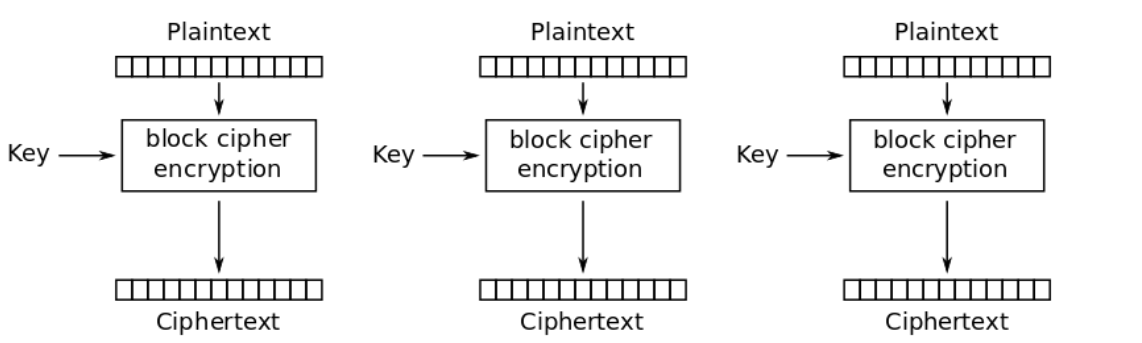
\includegraphics[width=\textwidth]{img/ecb.png}
    \par}

    Viene usato direttamente il \textit{block cipher}, è necessario utilizzare un informazione con lunghezza multipla della \textit{block size} il dato viene diviso in $n$ blocchi e successivamente cifrati tramite il blocco e gli $n$ blocchi di \textit{ciphertext} vengono concatenati, è molto inefficiente e \textbf{vulnerabile} (\textbf{\textit{ECB Penguin}}). \\
    In alcuni casi particolari viene comunque utilizzato, soprattuto per sviluppare e mantenere del codice.

    \textcolor{red}{\textbf{\textit{Mode of Operation - Counter Mode (CTR)}}}


    {\centering
        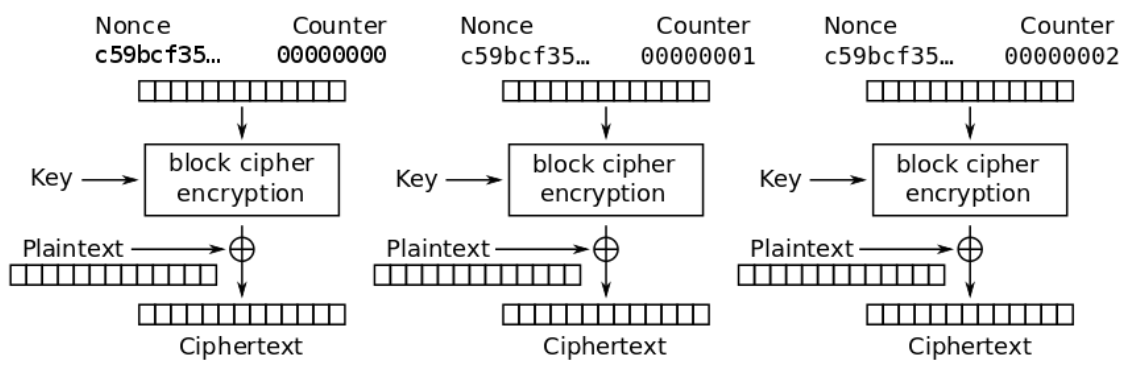
\includegraphics[width=\textwidth]{img/ctr.png}
    \par}

    Permette di costruire un \textbf{\textit{stream cipher}} da un \textit{block cipher}, dove il blocco viene utilizzato come funzione per generare bit pseudo-casuali (\textbf{\textit{stream key}}). È molto utilizzato nelle comunicazioni, è importante l'uso del \textbf{\textit{nonce}}. \\
    È importante andare ad analizzare il \textbf{\textit{nonce}}, infatti sappiamo che $len_n + len_c = b$ dove \textbf{b} è la \textit{block size} come bilanciamo la \textbf{lunghezza} del \textbf{\textit{nonce}} ($len_n$) e la \textbf{lunghezza} del \textbf{\textit{counter}} ($len_c$). Ipotizziamo di utilizzare \textbf{AES} come \textit{block cipher} e fissiamo $len_n = 64$ avremo problemi di \textbf{ricorsione statistica} dopo:
    
    {\centering
        $2^{len_c} \cdot 2^{\log_2 b} = 2^{64} \cdot 2^7 = 2^{71}$
    \par}

    Andando ad aumentare $len_n = 96$ avremo invece problemi di ricorsione dopo $2^{39}$ bytes $\simeq$ 64gb. La lunghezza del \textbf{\textit{nonce}} va a modificare il \textbf{numero di messaggi} prima che ci siano problematiche legate alla crittoanalisi statistica, mentre la lunghezza del \textbf{\textit{counter}} va a modificare la \textbf{grandezza del messaggio} prima che al suo interno possano esserci problematiche legate alla crittoanalisi statistica.

    \textcolor{red}{\textbf{\textit{Mode of Operation - Cipher Block Chaning (CBC)}}}


    \begin{figure}[h]
        \centering
        \begin{minipage}[t]{0.45\textwidth}
            \centering
            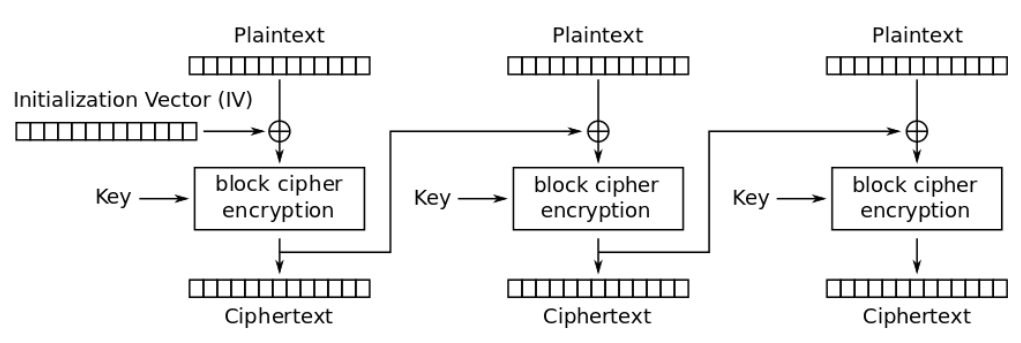
\includegraphics[width=\textwidth]{img/cbc_enc.png}
            \caption{\textbf{CBC \textit{encryption}}}
        \end{minipage}
        \begin{minipage}[t]{0.45\textwidth}
            \centering
            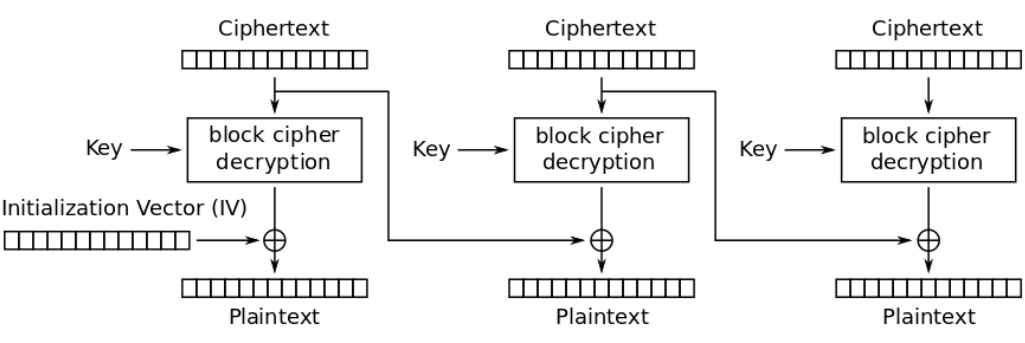
\includegraphics[width=\textwidth]{img/cbc_dec.png}
            \caption{\textbf{CBC \textit{decryption}}}
        \end{minipage}
    \end{figure}
    Il \textbf{CBC} usa il blocco cifrato precedente ottenendo così un \textbf{effetto a valanga} (\textit{avalanche effect}) questo porta ad avere a parità di blocchi di testo in chiaro differenti blocchi di crittogramma. Aumenta, inoltre, la resistenza contro attacchi del tipo di \textbf{\textit{frequency analysis}} questo non rimuove l'utilità di modifica nel tempo della chiave (\textbf{\textit{re-keying}} è comunque importante dopo una certa quantità di dati cifrati).

    \bigskip

    Introduce l'utilizzo di un \textbf{\textit{Initialization Vector}} per abilitare \textbf{\textit{multi-message security}} (molto simile al \textit{nonce} ma si basa su assunzioni di sicurezza diversi). L'\textbf{IV} è un dato random non c'è bisogno di mantenerlo segreto.

    \bigskip

    Al contrario del \textbf{CTR} che è vulnerabile (come l'\textbf{OTP}) a \textbf{malleabilità} il \textbf{CBC} è abbastanza resistente, assumiamo che un attaccante abbia un \textbf{\textit{decryption oracle}} e posso modificare l'$n$-esimo blocco avremo controllo di modifica dell'$n$-esimo bit dell'$(n + 1)$-esimo blocco. Il \textbf{CBC} al contrario è molto più sensibile a problematiche legate a disturbi o malfunzionamenti della rete. Altre grande differenza è che a differenza del \textbf{CTR} che è \textbf{parallelizzabile} per entrambi le funzioni (\textit{encryption} e \textit{decryption}) il \textbf{CBC} no.

    \bigskip

    \textcolor{red}{\textbf{\textit{Re-Keying}}} è la pratica per cui dopo $\Delta$ messaggi inviati la chiave simmetrica deve cambiare, ma questa pratica è in mano al protocollo e non allo schema.

\end{flushleft}

\begin{flushleft}
    \textcolor{red}{\textbf{\textit{Multi-message Security}}} \\
    Dobbiamo considerare che gli \textit{encryption scheme} come un \textit{tool} \textbf{\textit{general purpose}}, normalmente ogni informazione può essere trasmessa come dati binario a lunghezza variabile e bisogna essere capaci di cifrare messaggi differenti con la stessa chiave senza che l'attaccante sia capace di distinguere se stiamo cifrando due messaggi uguali o differenti. Per questo motivo si è deciso di utilizzare o il \textbf{\textit{nonce (n)}} o il \textbf{\textit{initialization vector (iv)}}, anche se è un informazione pubblica devono essere scelti da un attore ``onesto'' non dall'attaccante, se così non fosse ci possono essere attacchi potenziali a strutture simmetriche. È anche importante ricordare che i \textit{block cipher} sono deterministici e che quindi utilizzando (nel caso del \textbf{CBC}) lo stesso \textbf{IV}, stesso \textit{plaintext} e stessa \textbf{chiave} avremo lo stesso \textbf{\textit{ciphertext}}.

    \bigskip

    Esistono altre \textbf{\textit{mode of operations}} oltre a \textbf{ECB}, \textbf{CTR}, \textbf{CBC} che affronteremo più avanti e che avranno a che fare con garanzie di \textbf{autenticazione}.
\end{flushleft}

\section[Section Title. Section Subtitle]{Opeation Framework for Symmetric Encryption\\ {\small Developer view to symmetric encryption}}

\textcolor{red}{\textbf{\textit{Operations Framework}}} $\leftrightarrow$ \textbf{\textit{interface}} anche note come \textbf{API} che vengono utilizzate per interagire con uno \textbf{schema} o \textbf{protocollo}.

\begin{center}
    \begin{tikzpicture}[
    node distance=0.9cm and 1.5cm,
    main/.style={font=\bfseries, align=center},
    category/.style={text=blue, font=\bfseries, align=center},
    detail/.style={font=\scriptsize, align=center}
    ]

    \node[main] (enc) {encryption scheme};

    \node[category, below left=of enc] (interface) {interface};
    \node[category, below=of enc] (functional) {functional};
    \node[category, below right=of enc] (security) {security};

    \node[detail, below=0.2cm of interface] (interfaceDetail) {deterministic vs. random};
    \node[detail, below=0.2cm of functional] (functionalDetail) {stream vs. block};
    \node[detail, below=0.2cm of security] (securityDetail) {initialization vector vs. nonce};

    % Arrows
    \draw[->, red, thick] (enc) -- (interface);
    \draw[->, red, thick] (enc) -- (functional);
    \draw[->, red, thick] (enc) -- (security);

    \end{tikzpicture}
\end{center}

\begin{flushleft}
    Alcune interfacce non espongono un \textbf{API} che non richiede \textbf{IV} o \textbf{nonce}, ma lo generano internamente, quindi a pari input possono esistere più output. Questo è stato scelto per evitare che nel ``mondo reale'' \textbf{IV} e \textbf{nonce} vengono spesso confusi ed esposti nelle interfacce in maniera invertibile, questa cosa è molto pericolosa in quanto hanno requisiti differenti:
    \begin{itemize}[nosep]
        \item nel caso del \textit{nonce} è fondamentale l'\textbf{unicità}.
        \item nel caso del \textit{iv} è fondamentale la \textbf{randomicità}.
    \end{itemize}
    In alcuni casi è possibile utilizzare un \textit{nonce} per generare un \textit{iv}. 

    \bigskip

    Il \textit{nonce} a volte ci serve generali ``a mano'' infatti generandolo in maniera random esiste la possibilità dopo un certo numero $n$ di iterazioni della cifratura la possibilità di duplicarlo. Generandoli ``a mano'', ad esempio con un \textbf{contatore}, si ha la garanzia di utilizzare tutti i possibili valori dello spazio, ad esempio considerando un \textit{nonce} a 96 bit, se utilizzo un contatore il \textit{nonce} avrà tutti i possibili valori da $0$ a $2^{96} - 1$ prima di avere un duplicato. Il \textbf{NIST - \textit{National Institute of Standard Technology}} definisce la probabilità massima con la quale può avvenire una duplicazione del \textit{nonce} andando a basarsi sulla lunghezza dello stesso: $p = 2^{-32}$.
    \begin{itemize}[nosep]
        \item se uso un contatore (\textbf{\textit{statefull}}) allora ho $2^{96}$ combinazioni da utilizzare.
        \item se uso un random (\textbf{\textit{stateless}}) allora ho $2^{32}$ combinazioni prima di trovarmi nella condizione di \textbf{\textit{nonce} duplicati}.
    \end{itemize}

    \textcolor{red}{\textbf{\textit{SIV - Syntetic Initialization Vector}}}: è un modo per ottenere metodi alternativi il \textit{nonce} dall'\textit{iv} e viceversa, oppure è possibile cambiare schema di cifratura.

    \bigskip

    \textcolor{red}{\textbf{\textit{Encryption \& Padding}}} \\
    Siccome bisogna essere capaci di cifrare dati che hanno una lunghezza non multipla della \textit{block size}, abbiamo la necessità di aggiungere informazioni fittizie per raggiungere la lunghezza richiesta: \textbf{\textit{padding}}. L'unico requisito è che sia distinguibile dal contenuto reale. \\
    \textcolor{red}{\textbf{\textit{PKCS\#7}}}: aggiunge $n$ volte il valore $n$ per tutto il numero di bytes che mancano, nel caso in cui i dati sono già in lunghezza multipla della \textit{block size} allora bisogna aggiungere un blocco intero di padding.
\end{flushleft}